\todo[inline,author=Tiffani]{Качество картинок в главе не очень.}

В этом разделе мы рассмотрим колебания токов (зарядов, напряжений) в
электрических цепях, включающих в себя резисторы, конденсаторы и катушки
индуктивности. Это --- свободные затухающие колебания в колебательном контуре, а
также вынужденные установившиеся колебания, возбуждаемые внешней ЭДС,
изменяющейся по синусоидальному закону. Изложение материала будет ориентировано
на его применение в лабораторном практикуме. Более детальное рассмотрение
электрических колебаний можно найти, например, в работах [1~--~5], ссылки на
которые даны в конце раздела.

Все колебания мы будем рассматривать при относительно низких частотах, когда
выполняется условие квазистационарности. Квазистационарность означает, что в
каждый момент времени значения тока~$I$ практически одинаковы во всех элементах
цепи, соединённых последовательно, то есть изменения токов во времени происходят
настолько медленно, что распространение электродинамических взаимодействий,
которое происходит со скоростью, близкой к скорости света в вакууме~$c$, можно
считать \important{мгновенным}. Условие квазистационарности выполнено, если
время~$\Delta t$ распространения электромагнитного возмущения на расстояние~$l$,
характеризующего геометрические размеры цепи, много меньше периода~$T$ колебаний
тока в контуре: $\Delta t=l/c\ll T$, или частота колебаний $\nu=1/T\ll1/\Delta
t$. Практически длина~$l$ совпадает с длиной провода, из которой изготовлена
обмотка катушки индуктивности. При $l=1$~м условие квазистационарности хорошо
выполняется при частотах $\nu\ll3\cdot10^8$~Гц.

Выполнение условия квазистационарности позволяет при расчёте цепей переменного
тока использовать закон Ома для замкнутой цепи и закон сохранения заряда так же,
как и при расчёте цепей постоянного тока. Следствием этих двух законов являются
два правила Кирхгофа. Первое правило: в каждой точке разветвления проводов
алгебраическая сумма токов равна нулю. Второе правило: для любого замкнутого
контура сумма падений напряжений на отдельных участках равна алгебраической
сумме ЭДС в этом контуре.

Ниже мы будем рассматривать, в основном, идеализированные цепи переменного тока,
в которых всё омическое сопротивление сосредоточено в резисторе,
некомпенсированные заряды расположены только на обкладках конденсатора, а всё
магнитное поле, связанное с током в цепи, локализовано в катушке индуктивности.
Более детальный учёт омических потерь в конденсаторах и катушках индуктивности
будет проведён в описаниях лабораторных работ, посвящённых изучению колебаний в
цепях переменного тока, где эти потери могут играть заметную роль.

Условие квазистационарности позволяет использовать связь между током~$I$ и
напряжением~$U$ на каждом из трёх элементов стандартной цепи:
для резистора с сопротивлением~$R$ напряжение
\begin{equation}
	\eqmark{2.1}
	U_R=IR;
\end{equation}
для конденсатора с ёмкостью~$C$ (когда ток~$I$ направлен к положительно
заряженной пластине):
\begin{equation}
	\eqmark{2.2}
	I=\dfrac{dq}{dt}=C\dfrac{dU_C}{dt};
\end{equation}
для катушки самоиндукции с индуктивностью~$L$:
\begin{equation}
	\eqmark{2.3}
	U_L=L\dfrac{dI}{dt}.
\end{equation}

В случае цепей постоянного тока правила Кирхгофа дают возможность получить
полную систему линейных алгебраических уравнений, из решения которой могут быть
найдены все неизвестные токи (заряды, напряжения). При расчёте цепи переменного
тока, используя эти правила для произвольного момента времени, мы получаем
систему линейных дифференциальных уравнений, которые позволяют найти временную
зависимость токов (зарядов, напряжений) в данной цепи. В частном случае, когда
речь идёт о вынужденных стационарных колебаниях, нет необходимости каждый раз
решать дифференциальные уравнения: для этих случаев используется стандартный
метод комплексных амплитуд или метод векторных диаграмм. Оба эти метода будут
рассмотрены ниже в пункте <<Вынужденные колебания>>.

\introsection{Свободные колебания}

Рассмотрим электрический контур, состоящий из последовательно соединённых
резистора~$R$, конденсатора~$C$ и катушки индуктивности~$L$
(рис.~\figref{fig1}).

\begin{figure}[h!]
	\centering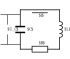
\includegraphics[width=0.3\linewidth]{Chapter_2/1}
	\caption{Колебательный контур.}
	\figmark{fig1}
\end{figure}
\todo[inline]{В старом тексте картинка такая же в лучшем качестве}


Сумма падений напряжения на элементах цепи в отсутствии внешней ЭДС равна нулю:
\begin{equation}
	\eqmark{2.4}
	RI+U_C+L\dfrac{dI}{dt}=0.
\end{equation}
Подставив в уравнение \eqref{2.4} выражения для~$I$ и $dI/dt$ из \eqref{2.2},
приходим к уравнению
\begin{equation}
	\eqmark{2.5}
	CL\dfrac{d^2U_C}{dt^2}+CR\dfrac{dU_C}{dt}+U_C=0.
\end{equation}
\todo[inline,author=Popov]{Промежуточные выкладки, на которые нет ссылки в тексте,
    должны идти без нумерации.}

Разделим это уравнение на~$CL$ и введём обозначения:
\begin{equation}\eqmark{2.6}
\gamma=\dfrac{R}{2L},~~~\omega_0^2=\dfrac{1}{LC},
\end{equation}
где $\gamma$~--- \important{коэффициент затухания},
$\omega_0$~--- \important{собственная круговая частота} колебательного контура.
Прилагательное  \important{<<круговая>>} в дальнейшем для сокращения записи
будем опускать. Введём также  \important{период собственных колебаний}~$T_0$:
\begin{equation}\eqmark{2.7}
T_0=\dfrac{2\pi}{\omega_0}=2\pi\sqrt{LC.}
\end{equation}
Уравнение для напряжения на конденсаторе~$U_C$ в колебательном контуре принимает
теперь вид:
\begin{equation}\eqmark{2.8}
\ddot{U}_C+2\gamma\dot{U}_C+\omega_0^2U_C=0,
\end{equation}
\todo[inline,author=Popov]{Выбор $U_C(t)$ в качестве основной величины
    сильно загромождает последующие выкладки. Почему бы не использовать
    заряд $q(t)$? Или обозначить просто $U(t)$?}
где точкой обозначено дифференцирование по времени. Легко показать, что так же
выглядят уравнения для других величин, характеризующих колебания в контуре.
Впрочем, решив уравнение \eqref{2.8}, можно получить выражение для тока~$I$ по
формуле \eqref{2.2}, заряда~$q$~--- по формуле~$q=CU_C$, а напряжений~$U_R$ и
$U_L$~--- по формулам \eqref{2.1} и \eqref{2.3}.

Отметим, что линейными дифференциальными уравнениями второго порядка вида
\eqref{2.8} описывается обширный класс колебательных систем как электрических,
так и механических. Механические колебания уже подробно изучались в рамках
семинарского и лабораторного практикумов, на что мы будем рассчитывать при
дальнейшем изложении, сокращая некоторые выкладки.

Для решения уравнения \eqref{2.8} введём новую переменную~$U(t)$, положив
\begin{equation}\eqmark{2.9}
U_C(t)=U(t)e^{-\gamma t}.
\end{equation}
\todo[inline,author=Popov]{Неудачное обозначение. Вместо $U(t)$ лучше $A(t)$ ---
    амплитуда колебаний.}
При этом из \eqref{2.8} получаем уравнение
\begin{equation}\eqmark{2.10}
\ddot{U}+\omega_1^2U=0,
\end{equation}
где
\begin{equation}\eqmark{2.11}
\omega_1^2=\omega_0^2-\gamma^2.
\end{equation}
В зависимости от соотношения между коэффициентом затухания~$\gamma$ и
собственной частотой~$\omega_0$ напряжение~$U_C$ по-разному меняется во времени.
Возможны три варианта, которые мы рассмотрим раздельно.

\introsubsection{Случай $0<\gamma<\omega_0$~--- затухающие колебания}
С учётом определений \eqref{2.6} условие реализации режима затухающих колебаний
в рассматриваемом $LCR$-контуре принимает вид:
\begin{equation}\eqmark{2.12}
0<R<2\sqrt{L/C}=2\rho=R_{\text{кр}},
\end{equation}
где введены ещё две характеристики колебательного контура:
\important{реактивное} или \important{волновое сопротивление} $\rho=\sqrt{L/C}$
и \important{критическое сопротивление} $R_{\text{кр}}$.
\todo[inline,author=Popov]{Колебательный контур --- квазистационарная система,
    в которой излучением и распространением волн пренебрегается.
    Термин ``волновое сопротивление'' для системы, в которой нет никаких волн~---
    не удачный. Кроме того, введение избыточной терминологии затрудняет восприятие текста.}
При выполнении условия
\eqref{2.12} из формулы \eqref{2.11} следует, что $\omega_1^2>0$ и, значит,
уравнение \eqref{2.10} описывает гармонические колебания величины $U(t)$ с
амплитудой~$U_0$, круговой частотой~$\omega_1$ и начальной фазой~$\varphi_0$:
\begin{equation}\eqmark{2.13}
U(t)=U_0\cos(\omega_1t+\varphi_0).
\end{equation}
Теперь с учётом формулы \eqref{2.9} для напряжения $U_C(t)$ на конденсаторе
можно записать решение исходного уравнения \eqref{2.8} в виде
\begin{equation}\eqmark{2.14}
U_C(t)=U_0e^{-\gamma t}\cos(\omega_1t+\varphi_0).
\end{equation}

В этом выражении, представляющем \important{затухающие колебания} напряжения на
конденсаторе $U_C(t)$, множитель $U_0e^{-\gamma t}$ перед периодической функцией
$\cos(\omega_1 t+\varphi_0)$ называется \important{амплитудой затухающих
колебаний}, а величина $\omega_1t+\varphi_0$~--- \important{фазой затухающих
колебаний}. Выражение \eqref{2.14} содержит две постоянные интегрирования
дифференциального уравнения \eqref{2.8}: \important{начальную амплитуду}~$U_0$ и
\important{начальную фазу}~$\varphi_0$, определяемые начальными условиями
задачи, то есть значениями амплитуды и фазы~$U_C(t)$ при~$t=0$. Величина
\begin{equation}\eqmark{2.15}
\omega_1=\sqrt{\omega_0^2-\gamma^2}
\end{equation}
в этом случае представляет \important{круговую частоту свободных}, или
\important{собственных, затухающих колебаний} (не путать с собственной частотой
$\omega_0$).

\todo[inline,author=Popov]{Выделить примеры отдельным стилем с мелким шрифтом.}
\begin{exmpl}
В качестве примера рассмотрим случай, когда в начальный момент $(t=0)$ ток в
контуре $I(0)=0$, а напряжение на конденсаторе $U_C(0)=U_{C0}$, то есть
конденсатор имеет заряд $q(0)=q_0=CU_{C0}$. С~учётом \eqref{2.15} и \eqref{2.2}
это означает, что для уравнения \eqref{2.8} приняты начальные условия
\begin{equation}
	\eqmark{2.16}
		\begin{gathered}[c]
			U_C(0)=U_{C0}=U_0\cos\varphi_0, \\
			\dot{U}_C(0)=I(0)/C=-\gamma
U_0\cos\varphi_0-\omega_1U_0\sin\varphi_0=0.
		\end{gathered}
\end{equation}

Второе из условий \eqref{2.16} показывает, что $\tg\varphi_0=-\gamma/\omega_1$
и, следовательно,
\begin{equation}\eqmark{2.17}
\cos\varphi_0=\pm\omega_1/\omega_0, \qquad \sin\varphi_0=\mp\gamma/\omega_0.
\end{equation}
Выбор знака здесь не ограничивает общности решения. Выберем верхние знаки в
\eqref{2.17}. В этом случае при положительной постоянной интегрирования~$U_0$
после замыкания цепи, как станет видно из приведённых ниже формул, будет
происходить разрядка конденсатора. Начальные амплитуда~$U_0$ и фаза~$\varphi_0$
затухающих колебаний напряжения $U_C(t)$ на конденсаторе в представлении
\eqref{2.14} выражаются теперь через заданное начальное значение напряжения на
конденсаторе $U_{C0}$ и характеристики контура~$\gamma$ и~$\omega_1$:
\begin{equation}\eqmark{2.18}
U_C(t)=U_0e^{-\gamma t}\cos(\omega_1t+\varphi_0), \;
U_0=(\omega_0/\omega_1)U_{C0}, \; \varphi_0=-\arctg(\gamma/\omega_1).
\end{equation}
Для тока~$I(t)$ в контуре с учётом \eqref{2.2} получаем выражение в
представлении вида \eqref{2.14}:
\begin{equation}\eqmark{2.19}
I(t)=I_0e^{-\gamma t}\cos(\omega_1t+\pi/2), \qquad I_0=U_0/\rho,
\end{equation}
где~$I_0$ и~$\pi/2$~--- начальные значения амплитуды $I_0e^{-\gamma t}$ и фазы
затухающих колебаний тока соответственно.
\end{exmpl}

\todo[inline,author=Popov]{Текст превращается в простыню. Нужна структура.}
\paragraph{Фазовые траектории.}
Заметим, что формулу \eqref{2.14} можно представить и в другом виде:
\begin{equation}\eqmark{2.20}
U_C(t)=e^{-\gamma t}(A\cos\omega_1 t+B\sin\omega_1 t),
\end{equation}
где две новые постоянные~$A$ и~$B$ связаны с постоянными~$U_0$ и~$\varphi_0$
соотношениями
\begin{equation}\eqmark{2.21}
A=U_0\cos\varphi_0, \qquad B=-U_0\sin\varphi_0.
\end{equation}
При этом окончательные формулы для напряжения~$U_C(t)$ и тока~$I(t)$, выраженные
через~$U_{C0}$ и характеристики контура, принимают вид:

\begin{equation}
	\eqmark{2.22}
		\begin{gathered}[c]
			U_C(t)=U_{C0}e^{-\gamma
t}[\cos\omega_1t+(\gamma/\omega_1)\sin\omega_1t], \\
			I(t)=C\dot{U}_C(t)
=-\left(U_{C0}/\rho\right)(\omega_0/\omega_1)e^{-\gamma t}\sin\omega_1t.
		\end{gathered}
\end{equation}
Из формул \eqref{2.22} следует параметрическое представление
\important{траектории системы на фазовой плоскости} переменных $U_C(t),
\dot{U}_C(t)=I(t)/C$. Задание этих двух величин полностью определяет состояние
системы в момент времени~$t$.

На рис.~\figref{fig2}a показаны \important{в безразмерных переменных}
зависимости \eqref{2.22} напряжения и тока в контуре от времени в режиме
свободных затухающих колебаний: сплошная линия $u(x)=U_C(x)/U_{C0}$, где
$x=(\omega_1/2\pi)t$, соответствует напряжению на конденсаторе $U_C(t)$, а
штриховая линия $j(x)=\rho I(x)/U_{C0}$~--- точку в контуре $I(t)$. На
рис.~\figref{fig2}б показана фазовая траектория этих колебаний на плоскости
переменных   $u(x),~j(x)$, представляющая собой скручивающуюся спираль.

\begin{figure}[h]
	\begin{minipage}[h]{0.5\linewidth}
		\center{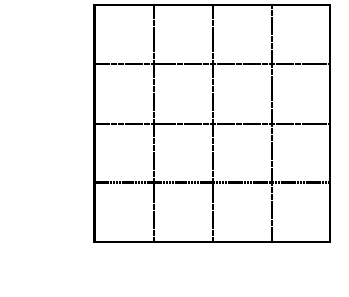
\includegraphics[width=1\linewidth]{Chapter_2/2} \\ а)}
	\end{minipage}
	\hfill
	\begin{minipage}[h]{0.5\linewidth}
		\center{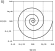
\includegraphics[width=0.9\linewidth]{Chapter_2/3} \\ б)}
	\end{minipage}
	\caption{(а,б). Затухающие колебания $(0<\gamma<\omega_0)$ при
$\gamma/\omega_0=0,1$.}
	\figmark{fig2}
\end{figure}

Из формул \eqref{2.14}, \eqref{2.19} и рис.~\figref{fig2} видно, что затухающие
при условии $0<\gamma<\omega_0$ колебания напряжения и тока не являются
периодическими функциями времени, однако эти величины дважды за время
\begin{equation}\eqmark{2.23}
T_1=\dfrac{2\pi}{\omega_1}=\dfrac{T_0}{\sqrt{1-\gamma^2/\omega_0^2}}
\end{equation}
проходят через нуль. А~так как согласно \eqref{2.2} нули функции $I(t)$ являются
нулями функции $dU_C/dt$, то величина~$T_1$ представляет также время между двумя
последовательными прохождениями напряжения $U_C(t)$ через максимум (минимум).
Очевидно, что экстремумы функции $I(t)$ чередуются с тем же периодом~$T_1$. Из
этих результатов возникает (с понятной долей условности) основание назвать
величину~$T_1$, определяемую формулами \eqref{2.23}, \important{периодом
затухающих колебаний}.

Взаимное расположение нулей и экстремумов $I(t)$ и~$U_C(t)$ легко понять из
энергетических соображений. Действительно, запасённая в контуре электромагнитная
энергия заключена в электрическом поле конденсатора и магнитном поле катушки
индуктивности, так что максимумы электрической энергии (экстремумы $U_C(t)$)
достигаются в нулях $I(t)$, а максимумы магнитной энергии (экстремумы $I(t)$)
достигаются в нулях $U_C(t)$.

Отметим, что все экстремумы не находятся на серединах временных интервалов между
соответствующими нулями, а сдвинуты влево на некоторую величину, возможность
определить которую предоставляется читателю.

Из формулы \eqref{2.23} следует, что $T_1>T_0$, то есть наличие потерь в
контуре, обусловленных сопротивлением~$R$ и представленных коэффициентом
$\gamma$, приводит к увеличению периода (уменьшению частоты) колебаний.

\todo[inline,author=Popov]{Текст превращается в простыню. Нужна структура.}
\paragraph{Характеристики затухающих колебаний.}
В~качестве характеристик процесса затухания колебаний помимо коэффициента
затухания~$\gamma$ используют \important{время затухания}
\begin{equation}\eqmark{2.24}
\tau=1/\gamma=2L/R,
\end{equation}
то есть время, за которое амплитуда колебаний убывает в~$e$ раз, а также
\important{логарифмический декремент}
\begin{equation}\eqmark{2.25}
\Theta=\ln\dfrac{U_{Ck}}{U_{C(k+1)}}=\ln e^{\gamma T_1}=\gamma T_1,
\end{equation}
\todo[inline,author=Popov]{Обозначение $U_{Ck}$ слишком громоздкое.
    Почему бы не использовать $A_k$?}
где $U_{Ck}$ и~$U_{C(k+1)}$~--- два последовательные максимальные отклонения
рассматриваемой величины (в данном примере - напряжения на конденсаторе) в одну
сторону от оси абсцисс. Из формул \eqref{2.24}, \eqref{2.25} следует связь между
логарифмическим декрементом~$\Theta$ и числом полных колебаний $N=\tau/T_1$ за
время затухания~$\tau$:
\begin{equation}\eqmark{2.26}
\Theta=1/N.
\end{equation}
Таким образом, логарифмический декремент затухания $\Theta$ равен обратному
числу~$N$ периодов~$T_1$, за которое амплитуда колебаний падает в~$e$ раз.

На практике для определения~$\Theta$ удобно использовать отношение максимальных
отклонений, разделённых целым числом~$n$ периодов~$T_1$ (см.
рис.~\figref{fig2}). В~этом случае формула для~$\Theta$ принимает вид:
\begin{equation}\eqmark{2.27}
\Theta=\dfrac{1}{n}\ln\dfrac{U_{Ck}}{U_{C(k+n)}}.
\end{equation}

Формулы \eqref{2.25}~--~\eqref{2.27} показывают, что максимумы (минимумы)
функции $U_C(t)$ образуют убывающую геометрическую прогрессию со знаменателем
\begin{equation}\eqmark{2.28}
U_{C(k+1)}/U_{Ck}=e^{-\Theta}.
\end{equation}
Такую же прогрессию образуют и экстремумы функции $I_C(t)$.

Логарифмический декремент определяет \important{шаг спирали затухающего
колебания} на фазовой плоскости. Действительно, из формулы \eqref{2.28} следует,
что
\begin{equation}\eqmark{2.29}
U_{Ck}-U_{C(k+1)}=U_{Ck}\left(1-e^{-\Theta}\right).
\end{equation}
Рекомендуем читателю проверить, что кривые на рис.~\figref{fig2} соответствуют
$\gamma/\omega_0=0,1$.

С~логарифмическим декрементом связана ещё одна характеристика колебательного
контура~--- его \important{добротность}

\begin{equation}
	\eqmark{2.30}
		\begin{aligned}[c]
			Q&=\dfrac{\pi}{\Theta}=\dfrac{\pi}{\gamma T_1}=\pi
N=\frac{1}{2}\sqrt{\omega_0^2/\gamma^2-1} = \\
			&=\frac{1}{2}\sqrt{R_{\text{кр}}^2/R^2-1}=\sqrt{\rho^2/R^2-1/4}.
		\end{aligned}
\end{equation}

Как правило, о добротности говорят только тогда, когда добротность контура
достаточно велика, то есть $Q\gg1$. Такой добротностью обладают колебательные
контуры со \important{слабым} затуханием, представляющие большой практический
интерес. Для них вместо неравенств $0<\gamma<\omega_0$ и \eqref{2.12}
выполняются неравенства
\begin{equation}\eqmark{2.31}
0<\gamma\ll\omega_0,
\end{equation}
или, в терминах параметров контура,
\begin{equation}\eqmark{2.32}
0<R\ll2\sqrt{L/C}=2\rho=R_{\text{кр}}.
\end{equation}
Малость отношения $\gamma/\omega_0$ и связанных с ним характеристик контура:
\begin{equation}\eqmark{2.33}
\gamma/\omega_0=R/2\rho=R/R_{\text{кр}}\ll1,
\end{equation}
-- позволяет, пренебрегая вторыми и выше степенями в разложениях по этим малым
величинам, значительно упростить уже полученные формулы, например, \eqref{2.15},
\eqref{2.17}~--~\eqref{2.23}, \eqref{2.30}, и дальнейшие выкладки. Так, в этом
приближении можно заменить~$\omega_1$ и~$T_1$ соответственно на~$\omega_0$ и
$T_0$, связать добротность~$Q$ с другими характеристиками контура цепочкой
равенств
\begin{equation}\eqmark{2.34}
Q=\dfrac{\pi}{\gamma
T_0}=\dfrac{\omega_0}{2\gamma}=\dfrac{\tau\omega_0}{2}=\dfrac{\omega_0L}{R}
=\dfrac{1}{\omega_0CR}=\dfrac{1}{R}\sqrt{\dfrac{L}{C}}=\dfrac{\rho}{R},
\end{equation}
а напряжение на ёмкости и ток в контуре \eqref{2.22} представить в виде

\begin{equation}
	\eqmark{2.35}
		\begin{gathered}[c]
			U_C(t)=U_{C0}e^{-\gamma
                t}[\cos\omega_0t+\frac{\gamma}{\omega_0}\sin\omega_0t], \\
            I(t)=-\frac{U_{C0}}{\rho}e^{-\gamma t}\sin\omega_0 t.
		\end{gathered}
\end{equation}

\paragraph{Энергетический смысл добротности.}
В~энергетическом смысле добротность~$Q$ колебательной системы
(механической, электрической, оптической и т. д.) определяется как отношение
запасённой в ней энергии~$W_0$ к потере $\Delta W_1$ энергии за время $T/2\pi$, за
которое фаза колебания меняется на 1 радиан:
\begin{equation}\eqmark{2.36}
Q=\dfrac{W_0}{\Delta W_1}=2\pi\dfrac{W_0}{\Delta W_T},
\end{equation}
где  $\Delta W_T$~--- потеря энергии за период~$T$.
\todo[inline,author=Popov]{Не вполне ясно: мы доказываем энергетический смысл добротности
2.0.34 или определим новое понятие ``энергетической добротности''?}
При вычислении~$\Delta W_T$
воспользуемся формулами \eqref{2.22} для представленных на рис.~\figref{fig2}
затухающих колебаний в \emph{рассматриваемом} $LCR$-контуре. Тот факт, что
они получены для конкретных начальных условий ($U_C(0)=U_{C0}$, $I(0)=0$),
не скажется, естественно, на общности результата. Пусть в момент времени~$t_0$ ток
в контуре $I(t_0)=0$, а напряжение на конденсаторе экстремально: $U_C(t_0)=\pm
U_{C0}e^{-\gamma t_0}$. Тогда ток равен нулю и в момент $t_0+T_1$. В~эти моменты
времени в электрическом поле конденсатора сосредоточена вся энергия контура. При
этом потеря энергии
\begin{equation}
	\eqmark{2.37}
		\begin{gathered}[c]
			 \Delta W_T = W(t_0)-W(t_0+T_1)=(1-e^{-2\gamma T_1})W_0, \\
			 W_0 = e^{-2\gamma t_0}CU_{C0}^2/2.
		\end{gathered}
\end{equation}
\todo[inline,author=Popov]{Комбинация $CU_{C0}$ выглядит ужасно}

Формулы \eqref{2.37} справедливы и для моментов времени $t\ne t_0$, однако, как
уже говорилось выше при обсуждении нулей и экстремумов $I(t)$ и $U_C(t)$,
электромагнитная энергия в этом случае распределяется между конденсатором и
катушкой индуктивности, составляя в сумме величину $W(t)$.

В~случае \emph{слабого} затухания, когда выполняются неравенства
\eqref{2.31}, формулу \eqref{2.37} можно упростить. В~первом порядке по малому
параметру $\gamma/\omega_0 \Delta W_T\approx 4\pi(\gamma/\omega_0)W_0$, так что
\[
\Delta W_1=\frac{\Delta W_T}{2\pi}\approx \frac{2\gamma}{\omega_0}W_0.
\]
Для <<энергетической>>
добротности \eqref{2.36} теперь приходим к формулам \eqref{2.34}, полученным в
случае \emph{слабого} затухания из введённого в общем случае
\emph{затухающих} колебаний выражения для добротности \eqref{2.30}.

\introsubsection{Случай $\gamma=\omega_0$~--- критический режим}
В этом варианте параметры контура связаны соотношениями
\begin{equation}\eqmark{2.38}
R=R_{\text{кр}}=2\sqrt{L/C}=2\rho,
\end{equation}
а уравнение \eqref{2.10} и его решение принимают вид: $\ddot{U}=0,
U(t)=A_1+A_2t$. Соответственно, напряжение на конденсаторе
\begin{equation}\eqmark{2.39}
U_C(t)=(A_1+A_2t)e^{-\gamma t},
\end{equation}
где постоянные интегрирования~$A_1$ и~$A_2$ определяются начальными условиями
задачи. Если, как и в \important{варианте 1}, приняты начальные условия:
$U_C(0)=U_{C0}$, $I(0)=0$,~--- то для напряжения на конденсаторе и тока в
контуре с учётом формул \eqref{2.9} и \eqref{2.2} получаем выражения:
\begin{equation}\eqmark{2.40}
U_C(t)=U_{C0}(1+\gamma t)e^{-\gamma t}, \qquad
I(t)=-\frac{U_{C0}}{\rho}\gamma t e^{-\gamma t}.
\end{equation}

Отметим, что на практике этот режим, требующий строгого выполнения условия
$\gamma=\omega_0$, не может быть точно реализован и имеет значение как
пограничный между режимом затухающих колебаний и рассматриваемого далее режимом
апериодического затухания.

\introsubsection{Случай $\gamma>\omega_0$~--- апериодический режим}
В~этом режиме $\omega_1^2=\omega_0^2-~\gamma^2<~0$, так что для
описания системы удобно перейти от тригонометрических функций к гиперболическим
функциям, введя вместо мнимой теперь величины~$\omega_1$ действительную величину
\begin{equation}\eqmark{2.41}
\alpha=\sqrt{\gamma^2-\omega_0^2}=\omega_0\sqrt{R^2/R_{\text{кр}}^2-1.}
\end{equation}
С~помощью подстановки нетрудно убедиться, что общее решение уравнения
\eqref{2.10} имеет при этом вид $U(t)=B_1e^{\alpha t}+B_2e^{-\alpha t}$, где
постоянные величины~$B_1$ и~$B_2$ определяются начальными условиями.
Соответственно, напряжение на конденсаторе
\begin{equation}\eqmark{2.42}
U_C(t)=e^{-\gamma t}(B_1e^{\alpha t}+B_2e^{-\alpha t}).
\end{equation}
При начальных условиях $U_C(0)=U_{C0}, I(0)=0$
\begin{equation}
	\eqmark{2.43}
		\begin{gathered}[c]
			U_C(t)=U_{C0}e^{-\gamma t}[\ch \alpha t+(\gamma/\alpha)\sh \alpha
t], \\
I(t)=-\frac{U_{C0}}{\rho}\frac{\omega_0}{\alpha}e^{-\gamma t}\sh \alpha t.
		\end{gathered}
\end{equation}

Как видно из \eqref{2.41}, апериодический режим реализуется, если параметры
контура удовлетворяют условию
\begin{equation}\eqmark{2.44}
R>R_{\text{кр}}=2\sqrt{L/C}=2\rho.
\end{equation}

Графики, соответствующие формулам \eqref{2.43}, а также фазовая траектория
системы в апериодическом режиме показаны в безразмерных переменных на
рис.~\figref{fig3} (a, б). На рис.~\figref{fig2}a сплошная линия
$u(x)=U_C(x)/U_{C0}$, где $x=\alpha t$, соответствует напряжению на конденсаторе
$U_C(t)$, а штриховая линия $j(x)=\rho I(x)/U_{C0}$~--- току в контуре $I(t)$.
На рис.~\figref{fig3}б показана фазовая траектория этих колебаний на плоскости
переменных $u(x),~j(x)$   при $\gamma/\omega_0=1,1~$, представляющая собой
короткий отрезок спирали.

\begin{figure}[h]
	\begin{minipage}[h]{0.49\linewidth}
		\centering{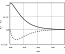
\includegraphics[width=1\linewidth]{Chapter_2/4} \\ а)}
		%\caption{а}
	\end{minipage}
	\hfill
	\begin{minipage}[h]{0.49\linewidth}
		\centering{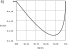
\includegraphics[width=0.9\linewidth]{Chapter_2/5} \\ б)}
		%\caption{б}
	\end{minipage}
	\caption{(а,б).Апериодический режим $(\gamma>\omega_0)$ при
$\gamma/\omega_0=1,1$.}
	\figmark{fig3}
\end{figure}

Как видно из рисунка, при выбранных начальных условиях в апериодическом режиме
на-пряжение на емкости убывает монотонно, а ток перед монотонным убыванием
совершает колебание, не меняя направления. Можно показать, что в этом режиме при
любых начальных условиях система стремится к равновесному состоянию
$U_C=0,~I=0$. При этом возможно не более одного прохождения через экстремальное
состояние, как на рис.~\figref{fig3}, и не более одного~--- через равновесное.

\introsection{Вынужденные колебания. Метод комплексных амплитуд. Векторные
диаграммы}

Рассмотрим процессы, протекающие в контуре, подключённом к источнику внешней
ЭДС, изменяющейся по гармоническому закону:
$\mathcal{E}=\mathcal{E}_0\cos(\omega t+\varphi_0)$. Соответствующая схема
представлена на рис.~\figref{fig4}.

\begin{figure}[h!]
	\centering
	\includegraphics[width=0.25\linewidth]{Chapter_2/6}
	\caption{Последовательный контур с внешней гармонической ЭДС}
	\figmark{fig4}
\end{figure}
\todo[inline,author=Popov]{Картинка совпадает с предыдущим изданием}

Потерями в конденсаторе и в катушке индуктивности в аналитических выкладках
будем пренебрегать, как и в п.1 при рассмотрении свободных колебаний. Потери в
катушке индуктивности учтём при рассмотрении векторных диаграмм.

Для напряжения на конденсаторе $U_C(t)$ вместо \eqref{2.8} получим теперь
уравнение
\begin{equation}\eqmark{2.45}
\ddot{U}_C+2\gamma \dot{U}_C+\omega_0^2U_C=\omega_0^2\mathcal{E}_0\cos(\omega t+
\varphi_0).
\end{equation}
Решение \important{линейного} дифференциального уравнения \eqref{2.45} с правой
частью состоит из общего решения однородного уравнения и какого-либо частного
решения данного уравнения с правой частью. Как показано в предыдущем разделе,
собственные свободные колебания контура (общее решение) при любых начальных
условиях экспоненциально затухают. Со временем их амплитуда становится
пренебрежимо малой, и в системе остаются только вынужденные колебания (частное
решение), обусловленные действием внешней ЭДС. Для нахождения этого частного
решения воспользуемся \important{методом комплексных амплитуд}. Данный метод
основан на следующем утверждении: \emph{пусть некоторая комплексная функция
является решением линейного дифференциального уравнения с вещественными
коэффициентами и комплексной правой частью; тогда вещественная часть этой
функции является решением того же уравнения, в правой части которого стоит
вещественная часть прежнего выражения, а мнимая часть~--- решением уравнения с
мнимой правой частью}.

Исходя из сказанного, перейдём к комплексному представлению колебаний и запишем
уравнение \eqref{2.45} в комплексной форме, отмечая комплексные величины
''стрелкой'':
\begin{equation*}
U_C=\Re \vec U_C, \quad \vec U_C=\Re \vec U_C+i\Im \vec U_C, \quad
\mathcal{E}=\Re \vec{\mathcal{E}}, \quad \vec{\mathcal{E}}=
\vec{\mathcal{E}}_0e^{i\omega t}=\mathcal{E}_0e^{i(\omega t+\varphi_0)},
\end{equation*}
\begin{equation}\eqmark{2.46}
\dfrac{d^2\vec U_C}{dt^2}+2\gamma\dfrac{d\vec U_C}{dt}+\omega_0^2\vec
U_C=\omega_0^2\mathcal{E}_0e^{i(\omega t+\varphi_0)}.
\end{equation}
Комплексная величина $\vec{\mathcal{E}}_0=\mathcal{E}_0e^{i\varphi_0}$, стоящая
перед $e^{i\omega t}$, называется \important{комплексной амплитудой} (в данном
случае это относится к внешней ЭДС). Решив уравнение \eqref{2.46}, мы получим
комплексное выражение для напряжения на конденсаторе. \important{Вещественная
часть} этого решения является, согласно приведённому выше утверждению, решением
исходного уравнения \eqref{2.45}.

Будем искать решение уравнения \eqref{2.46} в виде:
\begin{equation}\eqmark{2.47}
\vec U_C(t)=\vec U_{C0}e^{i\omega t},
\end{equation}
где $\vec U_{C0}$~--- комплексная амплитуда напряжения на конденсаторе, не
зависящая от времени. Подставляя \eqref{2.47} в \eqref{2.46} находим~$\vec
U_{C0}$, и далее, используя формулы \eqref{2.2}, \eqref{2.1},
\eqref{2.3},~--- комплексные амплитуды тока в контуре и напряжений на
сопротивлении и индуктивности:
\begin{subequations}
\renewcommand{\theequation}{\theparentequation \asbuk {equation}}
	\eqmark{2.48}
		\begin{equation}
			\eqmark{2.48a}
				\vec U_{C0}=(1/i\omega CZ)\mathcal{E}_0 e^{i\varphi_0}, \quad
Z=R+i(\omega L-1/\omega C)
		\end{equation}
		\begin{equation}
			\eqmark{2.48b}
			\begin{gathered}[c]
			\vec I_0=i\omega C\vec U_{C0}=(1/Z)\mathcal{E}_0 e^{i\varphi_0}, \\
			\vec U_{R0}=R\vec I_0=(R/Z)\mathcal{E}_0 e^{i\varphi_0}, \\
			\vec U_{L0}=i\omega L\vec I_0=(i\omega
L/Z)\mathcal{E}_0e^{i\varphi_0}
		\end{gathered}
		\end{equation}
\end{subequations}
\todo[inline,author=Popov]{Во всем разедел: сделать красивые формулы без лишних скобок.
    Сразу ввести обозначения так, чтобы громоздкие конструкции не возникали или
    хотя бы не повторялись.
Не выписывать лишний раз очевидные соотношения.}

Комплексная величина~$Z$ в формулах \eqref{2.48} называется
\important{комплексным сопротивлением}, или \important{импедансом},
последовательного контура и пишется обычно без ``стрелки``. Аналогичные
обозначения можно ввести и для отдельных элементов контура. Таким образом,
\begin{equation}
	\eqmark{2.49}
		\begin{gathered}[c]
			Z\equiv \Re  Z+i\Im Z=R+i(\omega L-1/\omega C), \\
			Z_R=R, \quad Z_L=i\omega L, \quad Z_C=-i/\omega C.
		\end{gathered}
\end{equation}
\todo[inline,author=Popov]{Здесь верхняя формула -- частный случай
    для последовательно соединённых RLC. Нижняя строка --- *общие*
    формулы для импедансов отдельных элементов каждого типа. Нужно разделить и подчеркнуть.}

В~этих обозначениях уравнения \eqref{2.48} принимают вид:
\begin{equation}
	\eqmark{2.50}
	\vec I_0=\vec{\mathcal{E}}_0/Z, \qquad \vec U_{R0}=Z_R\vec I_0, \qquad \vec
U_{C0}=Z_C\vec I_0, \qquad \vec U_{L0}=Z_L\vec I_0.
\end{equation}
Выражения \eqref{2.50} представляют обобщение закона Ома для переменных токов.
Роль сопротивлений в них играют импеданс контура~$Z$ в первом случае и импедансы
его отдельных элементов~--- в остальных случаях.

Важно отметить, что импеданс контура~$Z$ не зависит от начальных условий, не
содержит величин ни токов, ни напряжений, а определяется свойствами всех
элементов, соединённых в контур, и частотой синусоидальной ЭДС, к которой он
подключён. Таким образом, \important{импеданс~$Z$ является характеристикой
колебательного контура на заданной частоте}.

Выражение для~$Z$ содержит действительную часть $\Re Z=R$, называемую обычно
\important{активным сопротивлением} контура, и мнимую часть $\Im Z=\omega
L-1/\omega C$, носящую название \important{реактивного сопротивления}.
\emph{Правила сложения импедансов отдельных элементов схемы при
последовательном и параллельном включении~--- те же, что и для обыкновенных
сопротивлений}.

Импедансы реальных конденсаторов и катушек самоиндукции содержат кроме мнимой
части, также и действительную часть. Действительная часть импеданса определяется
необратимыми потерями энергии, которые могут быть связаны как с омическим
сопротивлением проводников, так и с другими причинами: с утечками и
диэлектрическими потерями в конденсаторах, с токами перемагничивания и токами
Фуко в магнитных сердечниках катушек самоиндукции. Потери в конденсаторах и в
катушках самоиндукции зависят как от частоты, так и от амплитуды проходящего
через них тока. Поэтому, приводя величины эквивалентного сопротивления потерь в
этих элементах, следует указывать частоту и амплитуду тока, при которых данные
величины были измерены.

Импедансы контура и его отдельных элементов~--- комплексные числа~--- могут быть
представлены в показательной форме. Для импеданса рассматриваемого
последовательного контура при этом находим:
\begin{subequations}
\renewcommand{\theequation}{\theparentequation \asbuk {equation}}
	\eqmark{2.51}
		\begin{equation}
			\eqmark{2.51a}
			Z=Z_0e^{i\psi_I}, \qquad Z_0=\sqrt{R^2+(\omega L-1/\omega
C)^2}=R/\cos\psi_I,
		\end{equation}
		\begin{equation}
			\eqmark{2.51b}
			\tg\psi_I=\Im Z/\Re Z=(\omega L-1/\omega C)/R, \quad
\psi_I=\arctg[(\omega L-1/\omega C)/R].
		\end{equation}
\end{subequations}
\todo[inline,author=Popov]{Обозначение $\psi_I$ ранее не определялось! Что это?}

Интересующие нас ток в контуре и напряжения на отдельных его элементах теперь
могут быть получены по формулам \eqref{2.48}~--- \eqref{2.50}. Например,
действительная часть тока в контуре
\begin{equation}
	\eqmark{2.52}
	I(t)=(\mathcal{E}_0/Z_0)\cos(\omega
t+\varphi_0-\psi_I)=(\mathcal{E}_0\cos\psi_I/R)\cos(\omega t+\varphi_0-\psi_I).
\end{equation}

Как видно из этой формулы, угол~$\psi_I$, определяемый отношением мнимой и
действительной частей импеданса, представляет собой сдвиг фаз между напряжением
на последовательном контуре и током в нём, причём \emph{положительные
значения угла~$\psi_I$ соответствуют отставанию фазы тока, а
отрицательные~--- опережению}. В~общем случае, когда к источнику последовательно
подключены резистор, конденсатор и катушка самоиндукции, сдвиг фазы тока
$\psi_I$ лежит в пределах $-\pi/2<\psi_I<\pi/2$. Из формулы \eqref{2.52} также
видно, что от угла~$\psi_I$ зависит амплитуда тока, а следовательно, и средняя
мощность активных потерь в контуре
\begin{equation}\eqmark{2.53}
	P=\langle I^2R\rangle_T=\mathcal{E}_0^2\cos^2\psi_I/2R,
\end{equation}
где угловые скобки с индексом <<$T$>> означают усреднение по периоду колебаний.
\todo[inline,author=Popov]{Все знают формулу с косинусом фи, а тут квадрат.
    Нужно как-то прокомментировать.

    Вообще стоит дать общий вывод связи мощности с комплексными амплитудами тока
    и напряжения. Эта формула важна и не очевидна. }

\todo[inline,author=Popov]{5 страниц текста без разбиения на структуру
    (позаголовки параграфов). Это не читаемо.}
\paragraph{Векторные диаграммы.}
Решения, полученные методом комплексных амплитуд, допускают простую
геометрическую интерпретацию. Комплексное число, например, напряжение
$\vec{\mathcal{E}}=\vec{\mathcal{E}}_0e^{i\omega t}=\mathcal{E}_0e^{i(\omega
t+\varphi_0)}$, представляется в комплексной плоскости вектором, длина которого
равна~$\mathcal{E}_0$~--- амплитуде напряжения $\mathcal{E}(t)$, а угол,
составляемый этим вектором с вещественной осью, равен $\omega
t+\varphi_0$~--- фазе напряжения $\mathcal{E}(t)$. Вектор $\vec{\mathcal{E}}$
вращается с угловой скоростью~$\omega$ против часовой стрелки. Удобно перейти к
системе координат, которая сама вращается с угловой скоростью~$\omega$. В~этой
системе вектор~$\vec{\mathcal{E}}$ будет представлен покоящимся вектором
$\vec{\mathcal{E}}_0=\mathcal{E}_0e^{i\varphi_0}$, а векторы~$\vec I_0$, $\vec U_{C0}$,
$\vec U_{R0}$ и~$\vec U_{L0}$ будут неподвижны, но окажутся сдвинутыми по углу
относительно вектора~$\vec{\mathcal{E}}_0$. Вектор~$\vec I_0$, как показано выше,
сдвинут от вектора~$\vec{\mathcal{E}}_0$ на угол~$\psi_I$, определяемый формулами
\eqref{2.51}.

Положения остальных векторов легко определить по формулам \eqref{2.48}. Так,
наличие множителя $i=exp(i\pi/2)$ в первом равенстве в \eqref{2.48b} означает,
что вектор~$\vec I_0$ опережает по углу на~$\pi/2$ вектор~$\vec U_{C0}$, то есть
ток опережает напряжение на конденсаторе по фазе на~$\pi/2$. Аналогично,
множитель $i=\exp(i\pi/2)$ в третьем равенстве в \eqref{2.48b} показывает, что
напряжение на индуктивности~$\vec U_{L0}$ опережает по фазе ток~$\vec I_0$ на
угол~$\pi/2$. Наконец, из второго равенства в \eqref{2.48b} видно, что вектор
$\vec U_{R0}$ совпадает по направлению с вектором~$\vec I_0$, и, значит,
напряжение на сопротивлении совпадает по фазе с током~$\vec I_0$. Построенные
таким образом диаграммы называются \important{векторными}.

В~качестве примера построим векторную диаграмму тока и напряжений для
последовательного контура. Рассмотрим схему, изображённую на рис.~\figref{fig5}.
К~источнику переменного напряжения $\mathcal{E}=\mathcal{E}_0\cos\omega t$
последовательно подключены резистор~$R$, катушка индуктивности~$L$,
действительная часть импеданса которой равна~$r_L$, и ёмкость~$C$. Активное
сопротивление~$r_L$ катушки индуктивности, которое с целью упрощения не
учитывалось выше при аналитическом решении задачи и будет учтено в описаниях
соответствующих лабораторных работ, легко может быть найдено в представленной на
рисунке <<схеме четырёх вольтметров>> с использованием векторной диаграммы.
Вольтметры измеряют напряжения на элементах цепи, амперметр измеряет ток.
Поскольку во всех элементах цепи ток~$I$ одинаков, удобно положить его фазу
равной нулю и отсчитывать от неё фазы напряжений на всех элементах цепи,
определив затем фазу   между напряжением на контуре и током.

\begin{figure}[h]
	\begin{minipage}[h]{0.37\linewidth}
		\centering{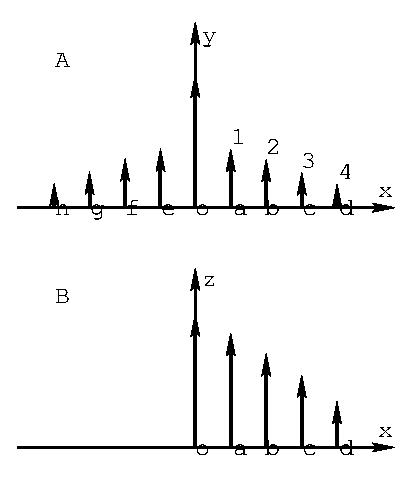
\includegraphics[width=1\linewidth]{Chapter_2/7} \\ а)}
		%\caption{а}
	\end{minipage}
	\hfill
	\begin{minipage}[h]{0.49\linewidth}
		\centering{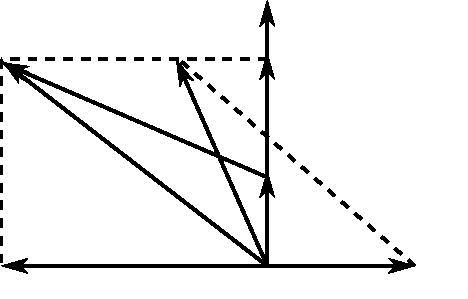
\includegraphics[width=1\linewidth]{Chapter_2/8} \\ б)}
		%\caption{б}
	\end{minipage}
	\caption{(а,б).Схема измерения (а) и векторная  диаграмма (б) для
последовательного контура}
	\figmark{fig5}
\end{figure}

Отложим вектор~$\vec I$ вдоль оси ординат (рис.~\figref{fig5}б). Напряжение на
резисторе совпадает по фазе с током, поэтому вектор~$\vec U_R$ также будет
направлен вдоль оси ординат. Напряжение на конденсаторе (без потерь) отстаёт по
фазе от тока на угол~$\pi/2$, поэтому вектор~$\vec U_C$ направлен
перпендикулярно вектору~$\vec I$ в сторону положительных значений абсцисс.
Векторное равенство напряжений $\vec U_{L+R}=\vec U_L+\vec U_R$ позволяет
построить треугольник по трём сторонам. Для этого сделаем две насечки:
первую~--- радиусом, равным модулю вектора $\vec U_{L+R}$, из начала этого
вектора (начала координат), вторую~--- радиусом, равным модулю вектора~$\vec
U_L$, из конца вектора~$\vec U_R$. Точка пересечения насечек определяет
положение векторов $\vec U_{L+R}$ и~$\vec U_L$ на диаграмме. Сложив векторы
$\vec{U}_{L+R}$ и~$\vec U_C$, получим вектор~$\vec{\mathcal{E}}$ входного
напряжения на контуре. Угол~$\psi_I$ показывает, каков сдвиг фаз между током и
напряжением в цепи. Разложим теперь вектор~$\vec U_L$ по осям координат.
Проекция~$\vec U_L$ на ось ординат позволяет определить $\vec
U_{L,\text{акт}}$~--- напряжение на активной части импеданса катушки, а проекция
на ось абсцисс даёт реактивную часть $\vec U_{L,\text{реакт}}$. Поделив эти
напряжения на ток~$I$, найдём действительную~$r_L$ и мнимую~$\omega L$ части
импеданса катушки.

\introsection{Вынужденные колебания. Резонанс}
\introsubsection{Резонанс напряжений в последовательном контуре}
В~предыдущем разделе были получены выражения \eqref{2.48}, описывающие в
комплексной форме вынужденные колебания в последовательном контуре под действием
внешней гармонической ЭДС. Там же указывалось, что эти колебания устанавливаются
в системе после затухания собственных свободных колебаний контура. Процесс
установления вынужденных колебаний будет рассмотрен отдельно в п.4 данного
раздела. Для исследования вынужденных колебаний и резонанса запишем
\important{вещественные части} решений \eqref{2.48}, использовав формулы
\eqref{2.7} и \eqref{2.12} для собственной частоты~$\omega_0$ и волнового
сопротивления~$\rho$, а также положив для сокращения записи раной нулю начальную
фазу:~$\varphi_0=0$. В~результате приходим к уравнениям:
\begin{subequations}
\renewcommand{\theequation}{\theparentequation \asbuk {equation}}
	\eqmark{2.54}
		\begin{equation}
			\eqmark{2.54a}
			I(t)=U_R(t)/R=I_{\omega}\cos(\omega t-\psi_I), \qquad
I_{\omega}=\mathcal{E}_0/Z_0,
		\end{equation}
		\begin{equation}
			\eqmark{2.54b}
			\begin{gathered}[c]
			Z_0=R\sqrt{1+(\rho/R)^2(\omega/\omega_0-\omega_0/\omega)^2},\\
			\psi_I=\arctg[(\rho/R)(\omega/\omega_0-\omega_0/\omega)],
			\end{gathered}
		\end{equation}
		\begin{equation}
			\eqmark{2.54c}
			U_C(t)=U_{C\omega}\cos(\omega t-\psi_C), \qquad
U_{C\omega}=\mathcal{E}_0\dfrac{\rho}{Z_0}\dfrac{\omega_0}{\omega}, \qquad
\psi_C=\psi_I+\pi/2,
		\end{equation}
		\begin{equation}
			\eqmark{2.54d}
			U_L(t)=U_{L\omega}\cos(\omega t-\psi_L), \qquad
U_{L\omega}=\mathcal{E}_0\dfrac{\rho}{Z_0}\dfrac{\omega}{\omega_0}, \qquad
\psi_L=\psi_I-\pi/2.
		\end{equation}
\end{subequations}
\todo[inline,author=Popov]{Нужно ли приводить ВСЁ это? Продраться через это невозможно.}

Отметим, что аналитическое выражение из \eqref{2.54b} для фазового сдвига
$\psi_I$ между внешней ЭДС и током в контуре легко упрощается в наиболее
интересной области, лежащей вблизи собственной частоты контура~$\omega_0$, а
фазовые сдвиги~$\psi_C$ и~$\psi_L$ связаны с~$\psi_I$ простыми соотношениями из
\eqref{2.54c} и \eqref{2.54d}. Напомним также, что согласно формуле \eqref{2.53}
от угла~$\psi_I$ зависит средняя мощность активных потерь в контуре.

Следует, однако, подчеркнуть, что в выражениях \eqref{2.54} не учтены
<<паразитные>> индуктивности и емкости реактивных элементов схемы, а также
возможные потери энергии в них. Необходимые уточнения будут сделаны в описаниях
соответствующих лабораторных работ.

Важно также отметить, что <<по умолчанию>> в нашем рассмотрении пренебрегалось
внутренним сопротивлением источника ЭДС, то есть считалось, что он является
\important{генератором напряжения}, который по определению обладает
\important{нулевым внутренним сопротивлением}. В~этом случае амплитуда
$\mathcal{E}_0$ не зависит от меняющегося с частотой сопротивления
нагрузки~--- последовательного колебательного контура.

Анализ формул \eqref{2.54} позволяет сделать следующие выводы.

1) При заданных параметрах~$\mathcal{E}_0$ и~$\omega$ внешнего источника
напряжения зависимости амплитуд и фаз тока и напряжений в системе от
частоты~--- \important{амплитудные} и \important{фазовые характеристики
системы}~--- определяются двумя безразмерными величинами: $\rho/R$ и
$\omega/\omega_0$. Как следует из формул \eqref{2.33}, \eqref{2.34}, для контура
со \important{слабым} затуханием, для которого добротность $Q\gg1$, отношение
$\rho/R=Q$, как уже отмечалось выше.

2) Поведение системы носит резонансный характер: при $\omega=\omega_0$, когда
мнимая часть импеданса контура $\Im Z=0$ и, соответственно,
%\setcounter{equation}{54}
\begin{equation}\eqmark{2.55}
	\omega_0L=1/\omega_0C=\rho,
\end{equation}
подкоренные выражения в формулах для амплитуд принимают минимальное значение,
равное единице, амплитуды тока и напряжения на сопротивлении достигают
максимальных значений
\begin{equation}\eqmark{2.56}
	I_{\omega_0}=\mathcal{E}_0/R, \qquad
U_{R\omega_0}=RI_{\omega_0}=\mathcal{E}_0
\end{equation}
и совпадают по фазе с ЭДС, поскольку~$\psi_0$. Таким образом, последовательный
контур на собственной частоте~$\omega_0$ представляет для внешней ЭДС чисто
активную нагрузку, на которой согласно \eqref{2.53} выделяется мощность
$P_{max}=\mathcal{E}_0^2/2R$.

3) Наиболее ярко резонансный характер вынужденных колебаний в
\important{последовательном} контуре проявляется в напряжениях на конденсаторе и
индуктивности, которые при $\omega=\omega_0$ в $\rho/R$ раз превышают напряжение
$\mathcal{E}_0$ по амплитуде и сдвинуты по фазе от него на $\mp\pi/2$
соответственно и, значит, находятся в противофазе друг с другом. Последние
утверждения, правда, относятся к идеальному случаю отсутствия потерь в этих
элементах. При добротности $Q=\rho/R\gg1$ амплитуды напряжений $U_C(t)$ и
$U_L(t)$ значительно превышают амплитуду~$\mathcal{E}_0$ напряжения на контуре.
По этой причине резонанс в последовательном контуре называется
\important{резонансом напряжений}.

4) Наличие множителей   в формулах \eqref{2.54c}, \eqref{2.54d} приводит к тому,
что \important{максимумы} напряжений на конденсаторе и индуктивности равны друг
другу, превышают $(\rho/R)\mathcal{E}_0$ и сдвинуты в разные стороны от
собственной частоты контура~$\omega_0$, на которой достигаются максимумы тока и
напряжения на сопротивлении~$R$:
\begin{equation}
	\eqmark{2.57}
	\begin{gathered}[c]
U_{C\omega_\text{m}}=U_{L\omega_\text{m}}=(\rho/R)\mathcal{E}_0[1-1/4(\rho/R)^2]
^{-1/2},\\
		\omega_{\text{m},C,L}=\omega_0[1-1/2(\rho/R)^2]^{\pm1/2}.
	\end{gathered}
\end{equation}
\todo[inline,author=Popov]{Может лучше так: $\mathcal{E}_0 \frac{Q}{\sqrt{1-Q^2/4}}$?
    И так везде.}
Рекомендуем читателям убедиться в этом самостоятельно.

Частоты, на которых достигаются \emph{максимальные} значения величин,
характеризующих вынужденные колебания в различных колебательных системах,
принято называть \important{резонансными}. Таким образом, в последовательном
колебательном контуре резонансной частотой для тока~$I$ и напряжения на
сопротивлении~$U_R$ является собственная частота контура~$\omega_0$, для
напряжения на конденсаторе~$U_C$~--- частота
$\omega_{\text{m}C}=\omega_0[1-1/2(\rho/R)^2]^{+1/2}$, для напряжения на
индуктивности~$U_L$~--- частота
$\omega_{\text{m}L}=\omega_0[1-1/2(\rho/R)^2]^{-1/2}$, причём
$\omega_{\text{m}C}\cdot\omega_{\text{m}L}=\omega_0^2$.

На рис.~\figref{fig6} приведены \important{в безразмерном виде} кривые
зависимостей от $x\equiv\omega/\omega_0$ амплитуды тока $j(x)\equiv
RI_\omega/\mathcal{E}_0$ (рис.~\figref{fig6} a) и амплитуды напряжения на
конденсаторе $u(x)\equiv U_{C\omega}/\mathcal{E}_0$  (рис.~\figref{fig6} б) при
трёх значениях отношения $\rho/R$, равных 2,~5 и 10.
\todo[author=Tiffani]{Нет подписи к рис. 2.6}
\begin{figure}[h]
	%\begin{center}
		\begin{minipage}[h]{0.45\linewidth}
			\centering{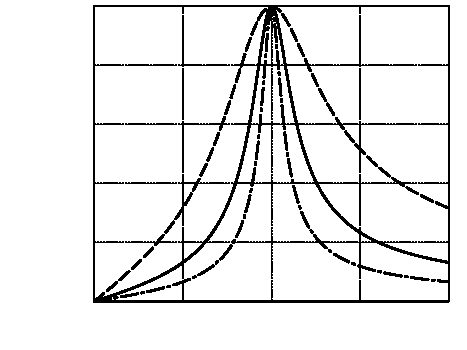
\includegraphics[width=1\linewidth]{Chapter_2/9} \\ а)}
			%\caption{а}
			%\figmark{fig6}
		\end{minipage}
		\hfill
		%\setcounter{figure}{5}
		\begin{minipage}[h]{0.45\linewidth}
			\centering{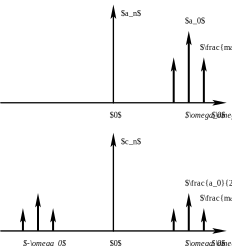
\includegraphics[width=1\linewidth]{Chapter_2/10} \\ б)}
			%\caption{б}
			%\figmark{fig9}
		\end{minipage}
	%\end{center}
		\caption{Нет подписи к рисунку}
		\figmark{fig6}
\end{figure}

Эти кривые называются \important{амплитудными резонансными кривыми}
колебательного контура. Важными характеристиками резонансных кривых являются
\important{максимальное значение амплитуды} соответствующей величины и
\important{ширина резонансной кривой}, при которой амплитуда этой величины
уменьшается в~$\sqrt{2}$ раз по сравнению со своим максимальным значением и в 2
раза уменьшается мощность сигнала. В~частности, по этим характеристикам можно
определить добротность колебательного контура. Например, эту величину можно
определить по отношению максимального значения напряжения на конденсаторе~$U_C$
к его статическому значению при~$\omega=0$, равному~$\mathcal{E}_0$, что следует
из формул \eqref{2.54} и видно из рис.~\figref{fig6}б.

Как уже отмечалось, о резонансе, как правило, говорят, если добротность~$Q$
колебательного контура достаточно велика и, следовательно, выполняются
соотношения \eqref{2.34}. Наибольший практический интерес представляет случай,
когда отклонение $\Delta\omega\equiv\omega-\omega_0$ частоты внешней ЭДС от
собственной частоты контура с добротностью $Q=\rho/R\gg1$ удовлетворяет сильному
неравенству
\begin{equation}\eqmark{2.58}
	|\Delta\omega|\ll\omega_0.
\end{equation}
При этом в первом порядке малости по \important{относительной расстройке
частоты} $\Delta\omega/\omega_0$
\begin{equation}\eqmark{2.59}
\dfrac{\omega}{\omega_0}-\dfrac{\omega_0}{\omega}=
\dfrac{2\Delta\omega}{\omega_0},
\end{equation}
что позволяет упростить выражения \eqref{2.54b} и представить их в виде:
\begin{subequations}
\renewcommand{\theequation}{\theparentequation \asbuk {equation}}
	\eqmark{2.60}
		\begin{equation}
			\eqmark{2.60a}
			Z_0=R\sqrt{1+(\tau\Delta\omega)^2}, \qquad
\psi_I=\arctg(\tau\Delta\omega),
		\end{equation}\\
		\text{где по определению \eqref{2.24} $\tau=1/\gamma$~--- время
затухания колебательного кон-}\\
		\text{тура.}\\
		\text{Соответственно упрощаются и выражения для амплитуд $I_{\omega}$,
$U_{C\omega}$ и $U_{L\omega}$ }\\
		\text{в остальных формулах \eqref{2.54}, в которые входит импеданс
контура $Z_0$:}
%костыль, но нормального работающего варианта со втавкой текста не придумала
		\begin{equation}
			\eqmark{2.60b}
			\begin{gathered}[c]
			I_{\omega}=\dfrac{\mathcal{E}_0}{R\sqrt{1+(\tau\Delta\omega)^2}},\\
U_{C\omega}=\dfrac{Q\mathcal{E}_0(\omega_0/\omega)}{\sqrt{1+(\tau\Delta\omega)^2
}},\\
U_{L\omega}=\dfrac{Q\mathcal{E}_0(\omega/\omega_0)}{\sqrt{1+(\tau\Delta\omega)^2
}}.
			\end{gathered}
		\end{equation}
\end{subequations}

На собственной частоте, когда $\omega=\omega_0,~\Delta\omega$, выражения для
амплитуд тока и напряжений на ёмкости и индуктивности, фазовых сдвигов и их
производных по частоте~$\omega$ принимают вид:
\begin{subequations}
\renewcommand{\theequation}{\theparentequation \asbuk {equation}}
	\eqmark{2.61}
		\begin{equation}
			\eqmark{2.54a}
			I_{\omega}(\omega_0)=U_{R\omega}(\omega_0)/R=\mathcal{E}_0/R, \qquad
\psi_I(\omega_0)=0,
		\end{equation}
		\begin{equation}
			\eqmark{2.54b}
			U_{C\omega}(\omega_0)=U_{L\omega}(\omega_0)=Q\mathcal{E}_0, \qquad
\psi_C(\omega_0)=-\psi_L(\omega_0)=-\pi/2,
		\end{equation}
		\begin{equation}
			\eqmark{2.54c}
			\psi'_I(\omega_0)=\psi'_L(\omega_0)=\psi'_C(\omega_0)=\tau.
		\end{equation}
\end{subequations}
Напомним, что максимальные (резонансные) значения напряжений на ёмкости и
индуктивности не строго равны~$Q\mathcal{E}_0$ и достигаются не строго на
частоте~$\omega_0$. Соответствующие относительные поправки, как это следует из
формул \eqref{2.57}, в рассматриваемом случае высокой добротности, когда
$Q\approx\rho/R\gg1$, составляют доли малой величины~$Q^{-2}$ и не учтены в
\eqref{2.61}.

\todo[inline,author=Popov]{Количество явно выписываемых формул нужно сократить. Очень трудно читать}

При отклонении $\Delta\omega=\omega-\omega_0=\Delta\omega{\gamma}$ таком, что
выполняется условие
%\setcounter{equation}{61}
\begin{equation}\eqmark{2.62}
\Delta\omega_{\gamma}=\pm\gamma, \quad \text{или} \quad
\tau\Delta\omega{\gamma}=\pm1,
\end{equation}
амплитуда тока~$I_{\omega}$, как видно из формул \eqref{2.60}, уменьшается в
$\sqrt{2}$ раз относительно своей максимальной (резонансной) величины, а фаза
$\psi_I$ изменяется на угол $\pm\pi/4$. Аналогичные изменения происходят с
амплитудами $U_{C\omega},~U_{L\omega}$ и фазами~$\psi_C$, $\psi_L$   напряжений на
ёмкости и индуктивности: амплитуды уменьшаются в~$\sqrt{2}$ раз, а фазы меняются
на угол~$\pm\pi/4$ по отношению к своим резонансным значениям.

Величина $\delta\omega\equiv2|\Delta\omega_{\gamma}|=2\gamma=2/\tau$
представляет собой важную характеристику колебательного
контура~--- \important{ширину резонансной кривой} $U_C(\omega)$, по которой с
учётом соотношений $Q=\omega_0/2\gamma=\tau\omega_0/2$ из \eqref{2.34}, зная
резонансную частоту~$\omega_0$, можно найти добротность контура
\begin{equation}\eqmark{2.63}
Q=\dfrac{\omega_0}{\delta\omega}.
\end{equation}

Ширину резонансной кривой и добротность можно определить и по
фазово-частотным характеристикам контура. Например, тангенс угла наклона
кривой $\psi_C(\omega)$ в точке резонанса согласно \eqref{2.54c} равен времени
затухания $\tau=2/\delta\omega$, а расстояние по оси~$\omega$ между точками, в
которых фаза~$\psi_C$ меняется от~$\pi/4$ до~$3\pi/4$, равно
$2/\tau=\delta\omega$.

Следует отметить, что в соотношении $\tau\cdot\delta\omega\sim1$, которому
подчиняется произведение времени затухания и ширины резонансной кривой
колебательного контура, проявляется фундаментальное \important{соотношение
неопределённости}, связывающее, в частности, <<время жизни>>~$\tau$ квантового
осциллятора с шириной спектральной линии~$\delta\omega$ его излучения (см.,
например, [1], с.~390).
\todo[inline,author=Popov]{Зачем квантового? В данном контексте это классическое
    соотношение для связи ширины спектра и длительности импульса. Дать ссылку на раздел 6}

\introsubsection{Резонанс токов в параллельном контуре}

Рассмотрим теперь вынужденные колебания в параллельном контуре, одна из ветвей
которого содержит индуктивность~$L$ и сопротивление~$R$, а другая~--- ёмкость
$C$ (рис.~\figref{fig7}).
\begin{center}
	\begin{figure}[h!]
		\centering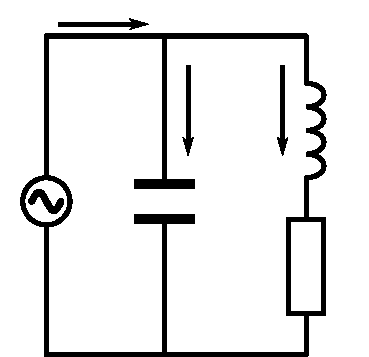
\includegraphics[width=0.25\linewidth]{Chapter_2/11}
		\caption{Параллельный контур с внешней гармонической ЭДС}
		\figmark{fig7}
	\end{figure}
\end{center}

Контур подключён к источнику ЭДС, задающему во внешней цепи ток, изменяющийся по
гармоническому закону: $I=I_0\cos(\omega t+\varphi_0)$. Таким образом, мы
предполагаем, что внутреннее сопротивлением источника столь велико, что он
является \important{генератором тока}, который по определению обладает
\important{бесконечно большим внутренним сопротивлением}. Потерями в катушке
индуктивности и конденсаторе будем пренебрегать, как это делалось и при
рассмотрении резонанса напряжений в последовательном контуре. Необходимые
уточнения будут сделаны в описаниях соответствующих лабораторных работ.

Воспользовавшись формулами \eqref{2.49}, правилами сложения сопротивлений и
правилами Кирхгофа, для комплексных амплитуд токов в ёмкостной~$\vec I_C$ и
индуктивной~$\vec I_L$ ветвях контура, а также для напряжения~$\vec U$ на
контуре, совпадающем в нашем приближении с напряжением на конденсаторе, при
начальной фазе $\varphi_0=0$ тока $\vec I=I_0e^{i\varphi_0}$ во внешней цепи
получаем выражения:
\begin{subequations}
\renewcommand{\theequation}{\theparentequation \asbuk {equation}}
	\eqmark{2.64}
		\begin{equation}
			\eqmark{2.64a}
			\vec I_C=\vec
I\dfrac{Z_{LR}}{Z_C+Z_{LR}}=i\dfrac{\rho\omega}{R\omega_0}I_0\dfrac{
1-iR\omega_0/\rho\omega}{1+i(\rho/R)(\omega/\omega_0-\omega_0/\omega)},
		\end{equation}
		\begin{equation}
			\eqmark{2.64b}
			\vec I_L=\vec
I\dfrac{Z_C}{Z_C+Z_{LR}}=-i\dfrac{\rho\omega_0}{R\omega}I_0\dfrac{1}{
1+i(\rho/R)(\omega/\omega_0-\omega_0/\omega)},
		\end{equation}
		\begin{equation}
			\eqmark{2.64c}
			\vec U=\vec IZ=\vec
I\dfrac{Z_CZ_{LR}}{Z_C+Z_{LR}}=\dfrac{\rho^2}{R}I_0\dfrac{
1-iR\omega_0/\rho\omega}{1+i(\rho/R)(\omega/\omega_0-\omega_0/\omega)},
		\end{equation}
\end{subequations}
где~$Z_C$ и~$Z_{LR}$~--- импедансы емкостной и индуктивной ветвей параллельного
контура соответственно.
\todo[inline,author=Popov]{Необходимо переобозначить и упростить. Либо не выписывать всё.}

Ограничимся рассмотрением наиболее интересного случая контура с высокой
добротностью вблизи резонансной частоты, когда $Q=\rho/R\gg1$, выполняется
условие \eqref{2.58} и применимо разложение \eqref{2.59}. При этом
\important{вещественные части комплексных амплитуд} \eqref{2.64} можно
представить в виде
\begin{subequations}
\renewcommand{\theequation}{\theparentequation \asbuk {equation}}
	\eqmark{2.65}
		\begin{equation}
			\eqmark{2.65a}
			I_C(t)=QI_0\dfrac{\omega}{\omega_0}\dfrac{\cos(\omega
t-\psi_C)}{R\sqrt{1+(\tau\Delta\omega)^2}}, \qquad
\psi_C=\arctg(\tau\Delta\omega)-\dfrac{\pi}{2}+Q^{-1},
		\end{equation}
		\begin{equation}
			\eqmark{2.65b}
			I_L(t)=QI_0\dfrac{\omega_0}{\omega}\dfrac{\cos(\omega
t-\psi_L)}{\sqrt{1+(\tau\Delta\omega)^2}}, \qquad
\psi_L=\arctg(\tau\Delta\omega)+\dfrac{\pi}{2},
		\end{equation}
		\begin{equation}
			\eqmark{2.65c}
			U(t)=Q\rho I_0\dfrac{\cos(\omega
t-\psi_U)}{\sqrt{1+(\tau\Delta\omega)^2}}, \qquad
\psi_U=\arctg(\tau\Delta\omega)+\dfrac{\omega_0}{\omega}Q^{-1}.
		\end{equation}
\end{subequations}

При резонансе, когда в принятом выше приближении
$\omega=\omega_0,~\Delta\omega=0$, амплитуды токов в ветвях контура, напряжения
на нём, фазовые сдвиги и их производные по циклической частоте~$\omega$
принимают вид:
\begin{subequations}
\renewcommand{\theequation}{\theparentequation \asbuk {equation}}
	\eqmark{2.66}
		\begin{equation}
			\eqmark{2.66a}
			I_{C\omega}=QI_0, \quad \psi_C(\omega_0)=-\dfrac{\pi}{2}+Q^{-1},
\quad I_{L\omega}(\omega_0)=QI_0, \quad \psi_L(\omega_0)=\dfrac{\pi}{2},
		\end{equation}
		\begin{equation}
			\eqmark{2.66b}
			U_{\omega}(\omega_0)=Q\rho I_0=Q^2RI_0, \qquad
\psi_U(\omega_0)=Q^{-1},
		\end{equation}
		\begin{equation}
			\eqmark{2.66c}
			\psi'_C(\omega_0)=\psi'_L(\omega_0)=\psi'_U(\omega_0)=\tau.
		\end{equation}
\end{subequations}
Из формул \eqref{2.63} следует, что на частоте~$\omega_0$ токи~$I_C$ и~$I_L$ в
ёмкостной и индуктивной ветвях контура в~$Q$ раз превышают ток~$I$ во внешней
цепи. При этом ток~$I_C$ опережает внешний ток~$I$ по фазе почти на~$\pi/2$, а
ток~$I_L$~--- отстаёт на~$\pi/2$. Между собой токи~$I_C$ и~$I_L$ сдвинуты по
фазе на угол, близкий к~$\pi$. Можно сказать, что токи~$I_C$ и~$I_L$ образуют
контурный ток, последовательно обтекающий элементы контура и в~$Q$ раз
превышающий по амплитуде внешний ток~$I$. Последнее обстоятельство послужило
поводом назвать резонанс в параллельном контуре \important{резонансом токов}.

Отметим, однако, что максимальные значения токов в контуре не строго равны
$QI_0$ и достигаются не строго на частоте~$\omega_0$. Соответствующие
относительные поправки, как и в случае резонанса напряжения, обусловлены
входящими в выражения \eqref{2.65}, \eqref{2.65b} для токов~$I_C$, $I_L$
множителями $(\omega_0/\omega)^{\pm1}$ и составляют доли малой величины
$Q^{-2}$.

Из формул \eqref{2.64b} вытекает, что на частоте~$\omega_0$ импеданс контура
$Z(\omega_0)=\vec U(\omega_0)/I_0$ является почти чисто активным. В
пренебрежении относительными поправками порядка~$Q^{-2}$ его модуль и фаза
относительно внешнего тока соответственно равны:
\setcounter{equation}{66}
\begin{equation}\eqmark{2.67}
|Z(\omega_0)|=Q\rho=Q^2R=\rho^2/R, \qquad \psi_Z(\omega_0)=Q^{-1}.
\end{equation}
Как видим, сопротивление контура в резонансе в~$Q^2$ раз превышает его активное
сопротивление~$R$. Это свойство параллельного контура широко используется в
радиотехнике.

По формулам \eqref{2.66a}, \eqref{2.66b} легко построить векторную диаграмму для
резонанса токов в рассмотренном выше параллельном контуре, в котором не
учитывались потери в конденсаторе и катушке индуктивности. Такая диаграмма
представлен на рис.~\figref{fig8}.

\begin{figure}[h!]
	\centering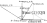
\includegraphics[width=0.5\linewidth]{Chapter_2/12}
	\caption{Векторная диаграмма при резонансе токов}
	\figmark{fig8}
\end{figure}

По оси ординат отложен внешний ток~$\vec I$. Напряжение на конденсаторе, равное
напряжению на контуре~$\vec U$, с учётом принятого правила знаков отстаёт по
фазе от тока~$\vec I$ на угол~$Q^{-1}$. Ток~$\vec I_C$ через конденсатор (без
потерь) опережает по фазе напряжение~$\vec U$ на~$\pi/2$. Ток через
индуктивность~$\vec I_L$ отстаёт от внешнего тока~$\vec I$ по фазе на~$\pi/2$.
Напряжение~$\vec U_R$ на сопротивлении совпадает по фазе с током~$\vec I_L$,
напряжение~$\vec U_L$ на индуктивности (без потерь) опережает ток~$\vec I_L$ на
$\pi/2$. Как видим, контур с активными потерями только в индуктивной ветви
проявляет ёмкостную реакцию: напряжение на контуре отстаёт по фазе от тока. Учёт
потерь в катушке индуктивности и конденсаторе несколько изменит векторную
диаграмму на рис.~\figref{fig8}, что будет рассмотрено в соответствующих
лабораторных работах.

Таким образом, условия резонанса токов в параллельном контуре и резонанса
напряжений в последовательном высокодобротном контуре совпадают:
$\omega=\omega_0$. Но, если в последовательном контуре резонансное сопротивление
контура равно чисто активному сопротивлению цепи~$R$ и минимально, обеспечивая
максимум тока при заданном внешнем напряжении, то в параллельном контуре
резонансное сопротивление контура почти чисто активное, обратно
пропорционально~$R$ и в~$Q^2$ раз его превышает, обеспечивая максимум напряжения
на контуре при заданном внешнем токе. Сдвиг фаз между напряжением и током при
резонансе напряжений всегда отсутствует, а при резонансе токов он близок к нулю
только, если $Q\gg1$. Впрочем, как правило, о резонансе и добротности говорят
только тогда, когда добротность контура достаточно велика.

\introsection{Установление вынужденных колебаний}

Рассмотрим процесс установления вынужденных колебаний в
\important{выскодобротном последовательном контуре}. Общее решение уравнения
\eqref{2.46} представляет собой сумму решения \eqref{2.14}, содержащего две
постоянные, зависящие от начальных условий задачи, и частного решения
\eqref{2.54c}. При наличии внешнего источника в качестве начальных естественно
выбрать <<нулевые>> условия: $U_C(0)=0,~\dot U_C(0)=0$, а решение искать в виде
\begin{equation}
	\eqmark{2.68}
	U_C(t)=U_{C\omega}\sin(\omega t-\psi_I)-U_0e^{-\gamma
t}\sin(\omega_1t-\varphi_0),
\end{equation}
где $U_{C\omega}$ и~$\psi_I$~--- зависящие от частоты~$\omega$ амплитуда и фаза
вынужденных колебаний, определяемые формулами \eqref{2.54}. Из начальных условий
при этом получаем систему уравнений, которая позволяет найти постоянные величины
$U_0$ и~$\varphi_0$:
\begin{equation}
	\eqmark{2.69}
	U_{C\omega}\sin\psi_I=U_0\sin\varphi_0, \qquad
U_{C\omega}\omega\cos\psi_I=U_0(\gamma\sin\varphi_0+\omega_1\cos\varphi_0).
\end{equation}
Для резонансного случая $\omega=\omega_0$, когда согласно \eqref{2.54}
$\psi_I=0$, а $U_{C\omega}=Q\mathcal{E}_0$, из уравнений \eqref{2.69} получаем
искомые константы $\varphi_0=0$ и $U_0=Q\mathcal{E}_0\omega_0/\omega_1$, а далее
из уравнения eqref{2.68}~--- \important{точное решение} задачи об установлении
вынужденных колебаний на резонансной частоте в последовательном контуре с
высокой добротностью при <<нулевых>> начальных условиях:
\begin{equation}
	\eqmark{2.70}
	U_{C}(t)=Q\mathcal{E}_0[\sin\omega_0t-(\omega_0/\omega_1)e^{-\gamma
t}\sin\omega_1 t].
\end{equation}
В общем случае при $\omega_1\approx\omega_0$ уравнение такого вида описывает
\important{биения} двух гармонических сигналов \important{близких} частот с
экспоненциально убывающей амплитудой одного из них. Появление биений связано с
тем, что разность фаз этих сигналов медленно меняется со временем:
$\Delta\varphi=(\omega_0-\omega_1)t$,~--- и при нулевой разности фаз сигналы
вычитаются друг из друга, а при расхождении фаз на~$\pi$
радиан~--- складываются. В~рассматриваемом случае \important{высокодобротного
контура}, в котором
$\gamma\ll\omega_0,~\omega_0-\omega_1\approx\gamma^2/2\omega_0$, набег фазы за
время $\tau=1/\gamma$ затухания свободных колебаний
$\Delta\varphi\approx(\gamma^2/2\omega_0)\tau=\gamma/2\omega_0\ll1$,  так что
биения не успевают проявиться. Процесс установления вынужденных колебаний на
резонансной частоте при этом можно представить в простейшем виде:
\begin{equation}\eqmark{2.71}
	U_C(t)=Q\mathcal{E}_0(1-e^{-\gamma t})\sin\omega_0 t.
\end{equation}

При отклонении частоты~$\omega$ внешней ЭДС от резонансной частоты
ограничимся, как и в п.3.1, рассмотрением наиболее интересного случая, когда
выполняется неравенство \eqref{2.58}, означающее, что мала относительная
расстройка частоты: $|\Delta\omega|/\omega_0\ll$. Тогда строгое решение первого
уравнения системы \eqref{2.69} имеет вид:
$\varphi_0=\psi_I,~U_0=\mathcal{E}_{\omega}$,~--- а второе из уравнений
\eqref{2.69} приводит к равенству $\gamma\tg\psi_I=\omega-\omega_1$, которое с
учётом \eqref{2.60} и \eqref{2.15} удовлетворяется с относительной погрешностью
$\approx0,1Q^{-2}$. Таким образом, в высокодобротном контуре при малой
относительной расстройке частоты внешней ЭДС установление вынужденных колебаний
подчиняется уравнениям
\begin{equation}
	\eqmark{2.72}
	\begin{gathered}[c]
U_C(t)=\dfrac{Q\mathcal{E}_0(\omega_0/\omega)}{\sqrt{1+(\tau\Delta\omega)^2}}[
\sin(\omega t-\psi_I)-e^{-\gamma t}\sin(\omega_0t-\psi_I)],\\
		\psi_I=\arctg(\tau\Delta\omega).
	\end{gathered}
\end{equation}
%\begin{equation}\eqmark{2.72}
%	U_C(t)=\dfrac{Q\mathcal{E}_0(\omega_0/\omega)}
%{\sqrt{1+(\tau\Delta\omega)^2}}[\sin(\omega t-\psi_I)-
%e^{-\gamma t}\sin(\omega_0t-\psi_I)],~~~~\psi_I=\arctg(\tau\Delta\omega).
%\end{equation}

Уравнения \eqref{2.72}, как и уравнение \eqref{2.70} в общем случае, описывают
биения двух гармонических сигналов близких частот с экспоненциально убывающей
амплитудой одного из них. При этом за время~$\tau$ затухания сигнала с частотой
$\omega_0$ разность фаз сигналов
$\Delta\varphi=\tau\Delta\omega=2\Delta\omega/\delta\omega$. Следовательно, при
расстройке $|\Delta\omega|\ll\delta\omega/2\ll\omega_0$, где, напомним,
$\delta\omega$~--- ширина резонансной кривой высокодобротного контура, биения
проявляться не будут, как и в резонансном случае, представленном уравнением
\eqref{2.67}. Установление вынужденных колебаний будет при этом проходить,
подчиняясь уравнению, подобному \eqref{2.71}:
\begin{equation}\eqmark{2.73}
	U_C(t)=Q\mathcal{E}_0(\omega_0/\omega)\left(1-e^{-\gamma
t}\right)\sin(\omega_0t-\tau\Delta\omega).
\end{equation}
Как видно из формул \eqref{2.71}, \eqref{2.73}, в случаях резонанса и малого
отклонения от него по сравнению с шириной резонансной кривой амплитуда
вынужденных колебаний со временем возрастает, экспоненциально приближаясь к
величине \\$Q\mathcal{E}_0(\omega_0/\omega)$, зависящей от частоты.

По полученной в эксперименте осциллограмме сигнала нетрудно определить
логарифмический декремент затухания~$\Theta$, период колебаний~$T_1$, близкий
$t_0=2\pi/\omega_0$, и рассчитать коэффициент затухания~$\gamma$ колебательного
контура. Проиллюстрируем эту процедуру, построив на рис.~\figref{fig9}
зависимость $U_C(t)$ по формуле \eqref{2.71}.

\begin{figure}[h!]
	\centering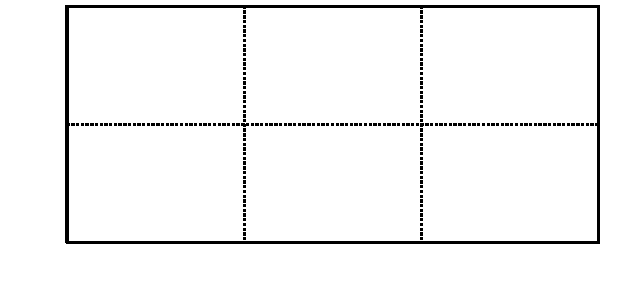
\includegraphics[width=0.6\linewidth]{Chapter_2/13}
	\caption{Установление колебаний вблизи резонанса
$(|\Delta\omega|\ll\gamma=\delta\omega/2)$}
	\figmark{fig9}
\end{figure}

Рассмотрим два момента времени~$t_1$ и~$t_2$, разделённые целым числом~$n$
периодов~$T_0$. Амплитуды колебаний $U_{Ck}(t_1)$ и $U_{C(k+n)(t_2)}$ при этом
соответственно равны:
\begin{equation}\eqmark{2.74}
U_{Ck}=U_0(1-e^{-\gamma t_1}), \qquad U_{C(k+n)}=U_0(1-e^{-\gamma(t_1+nT_0)}),
\qquad U_0=Q\mathcal{E}_0.
\end{equation}
Из этих выражений находим логарифмический декремент
\begin{equation}\eqmark{2.75}
\Theta=\dfrac{1}{n}\ln\dfrac{U_0-U_{Ck}}{U_0-U_{C(k+n)}}=\gamma T_0,
\end{equation}
а затем, измерив по осциллограмме реальный период $T_1\approx T_0$, определяем
коэффициент затухания~$\gamma$.

Если расстройка~$\Delta\omega$ удовлетворяет неравенствам
$|\Delta\omega|\approx\gamma=\delta\omega/2\ll\omega_0$, то есть расстройка
сопоставима с шириной резонансной кривой, установление вынужденных колебаний на
начальной стадии процесса длительностью~$\tau$ сопровождается биениями с
частотой $|\Delta\omega|=|\omega-\omega_0|$ согласно уравнениям \eqref{2.72}.
Вид колебаний в этом случае представлен на рис.~\figref{fig10}.

\begin{figure}[h!]
	\centering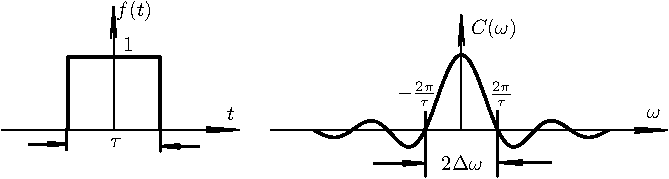
\includegraphics[width=0.6\linewidth]{Chapter_2/14}
	\caption{Биения при установлении колебаний
$(\Delta\omega\approx\gamma=\delta\omega/2)$}
	\figmark{fig10}
\end{figure}

Амплитуда колебаний при этом то растёт, то падает, причём максимумы амплитуд
постепенно уменьшаются. Лишь когда экспонента~$e^{-\gamma t}$ достаточно
затухнет, биения прекратятся, и колебания станут синусоидальными.
%\begin{center}
%СПИСОК ЛИТЕРАТУРЫ
%\end{center}

\introsection{Автоколебания}

\introsubsection{Автоколебания в системах с одной степенью свободы}
В предыдущих разделах были рассмотрены свободные и вынужденные колебания в
диссипативных системах с одной степенью свободы, подчиняющихся дифференциальным
уравнениям второго порядка вида \chaptereqref{2.8} и \chaptereqref{2.45}
соответственно. Диссипация энергии, обусловленная наличием резистивных элементов
в этих системах, в первом случае приводила к затуханию колебаний, а во
втором~--- компенсировалась энергией, поступающей от
внешнего источника синусоидального напряжения (или тока). Однако колебания в
системе с одной степенью свободы при определённых условиях можно поддерживать,
используя и \emph{постоянный} (не синусоидальный) источник энергии, 
который периодически компенсирует потери колебательной энергии по входящей 
в систему цепи \term{обратной связи}. 
Такие системы называются \term{автоколебательными}, а протекающие в
них процессы~--- \term{автоколебаниями}. Форма и период автоколебаний
определяются свойствами самой системы, чем автоколебания существенно отличаются
от обычных вынужденных колебаний

Для определения условий возбуждения автоколебаний в диссипативной системе с
одной степенью свободы воспользуемся уравнением изменения энергии 
системы \chaptereqref{JL}:
\begin{equation}
	\eqmark{auto-1}
	\frac{dW}{dt}=-P(t),
\end{equation}
где $W=\frac12 LI^2+ \frac{q^2}{2C}$~--- энергия, запасённая в колебательном контуре,
а $P(t)$~--- мощность потерь. 
Интегрируя \eqref{auto-1} по периоду колебаний $T$, приходим 
к равенству
\begin{equation}
	\eqmark{auto-2}
	W=W_0-\int\limits_{0}^{T}P(t)dt,
\end{equation}
где $W_0$~---~энергия системы в некоторый момент времени, принятый за начало
отсчёта. В обычной~--- диссипативной~--- системе $P(t)=RI^{2}(t)>0$, 
так что автоколебания невозможны. 
Если же мощность потерь $P(t)$ в системе можно сделать \important{знакопеременной}, 
то подбором режима работы системы можно обеспечить энергетический баланс:
\begin{equation}
	\eqmark{auto-3}
	\int\limits_{0}^{T} P(t) dt = 0,
\end{equation}
и, следовательно, возбудить в системе автоколебания. Отрицательные
<<потери>>, естественно, реализуются за счёт совершения 
работы внешним источником над системой.

Выполнение условия \eqref{auto-3} возможно, например, в \important{нелинейной}
колебательной системе, в которой сопротивление $R=\frac{dU}{dI}$ является 
функцией тока: $R=R(I)$, причём \emph{знакопеременной}. То есть для 
автоколебательного режима необходима возможность реализации
отрицательного \term{дифференциального сопротивления} цепи:
\[
R_{диф} = \frac{dU}{dI} < 0.
\]
Иными словами, вольт-амперная характеристика $I(U)$ элемента должна
обладать <<спадающими>> участками (участками с отрицательным наклоном). 
Примеры таких характеристик приведены на
рис.~\figref{auto-1}(а, б). Ими обладают, например, газоразрядная лампа 
(а) и туннельный диод (б). Обычно характеристики вида~(а) называют $S$-образными, 
а вида~(б)~---~$N$-образными.
\begin{figure}
	\centering
	\pic{0.8\textwidth}{Chapter_2/auto-1}
	%\import{Images/Chapter_2/}{auto-1.pdf_tex}
	\caption{Вольт-амперные характеристики с «падающими» участками: а)~$S$-образным, б) $N$-образным.}
	\figmark{auto-1}
\end{figure}

Форма автоколебаний зависит от добротности колебательного контура. При большой
добротности характер протекающих процессов почти не изменяется по сравнению с
тем, как они протекали бы в системе без поступления
энергии от источника: период и форма автоколебаний будут близки к периоду и
форме собственных колебаний. Это связано с тем, что в этом случае от постоянного
источника поступает энергия, составляющая малую
долю полной энергии колебательной системы. При малой добротности колебательной системы 
для поддержания колебаний от постоянного
источника должна поступать энергия, сопоставимая с энергией колебаний. В этом
случае форма автоколебаний может значительно отличаться от синусоидальной.
Наконец, в апериодической системе, в которой за период автоколебаний теряется вся
накопленная энергия, автоколебания становятся \term{релаксационными} и
могут по форме очень сильно отличаться от колебаний синусоидальных.

\introsubsection{Автоколебания в вырожденных системах}
Автоколебательная система, не содержащая одного из накопителей колебательной
энергии (например, индуктивности или емкости), называется \term{вырожденной}. Колебания в такой системе
описываются дифференциальным уравнением первого порядка и могут быть
только \emph{релаксационными}.

В качестве примера рассмотрим представленную на рис.~\figref{auto-2}(а,~б) 
вырожденную автоколебательную систему, содержащую источник
постоянного напряжения $U$, ёмкость $C$, сопротивление $R$ и нелинейный элемент
с $S$-образной вольт-амперной характеристикой $I_S(U)$. 

\begin{figure}[h]
	\begin{minipage}[h]{0.49\linewidth}
		\centering
		\pic{0.9\textwidth}{Chapter_2/auto-2}
		%\center{\resizebox{0.79\textwidth}{!}{\import{Images/Chapter_2/}{auto-2.pdf_tex}} \\ а) Схема автоколебательной $RC$-системы.}
	\end{minipage}
	\hfill
	\begin{minipage}[h]{0.49\linewidth}
		\centering
		\pic{0.79\textwidth}{Chapter_2/auto-3}
		%\center{\resizebox{0.79\textwidth}{!}{\import{Images/Chapter_2/}{auto-3.pdf_tex}} \\ б) Вольт-амперная характеристика и нагрузочная прямая $RC$-системы.}
	\end{minipage}
	\caption{Вырожденная автоколебательная $RC$-система}
	\figmark{auto-2}
\end{figure}

Уравнения, описывающие поведение этой системы релаксационного типа,
имеют вид:
\begin{equation}
	\eqmark{auto-4}
	RI+U=\mathcal{E},\quad I=I_C+I_S,\quad I_C=C\frac{dU}{dt},\quad I_S=I_S\left(U \right).
\end{equation}
Следовательно,
\begin{equation}
	\eqmark{auto-5}
	\tau_С\frac{dU}{dt}=\mathcal{E}-U-R{{I}_{S}}\left( U \right),
\end{equation}
где $\tau_С = RC$ --- характерное время разрядки конденсатора.

В стационарном состоянии, когда $dU / dt = 0$, должно выполняться равенство
\begin{equation}
	\eqmark{auto-6}
	I_S(U)=\frac{\mathcal{E}-U}{R}.
\end{equation}
Правая часть здесь представляет \important{нагрузочную прямую}, точки
пересечения которой с вольт-амперной характеристикой 
${I}_{S}\left( U \right)$ определяют стационарные состояния системы. 
На рис.~\figref{auto-2}б) параметры $\mathcal{E}$ и $R$ выбраны так, 
чтобы стационарное состояние $A(U_{А},\,I_{А})$ лежало на падающей
ветви вольт-амперной характеристики, где возможен автоколебательный режим. 

Покажем, что состояние $I_{А}=I(U_{А})$ может быть
\important{неустойчивым}. Для этого дадим малое приращение $\Delta U$ 
переменной $U$ в точке $U_{А}$ и представим в линейном приближении по 
$\delta U$ вольт-амперную характеристику $I_S(V)$ вблизи стационарного 
состояния $U_{А}$:
\begin{equation}
	\eqmark{auto-7}
I_S(U_{А} + \delta U)\approx 
    I_S(U_{А}) + {I}_S' \delta U,
\end{equation}
где ${I}_S' = \left.\frac{dI_S}{dU}\right|_{U_{А}}$ --- 
наклон вольт-амперной характеристики в точке~$U_{А}$. 
Подстановка этого выражения в \eqref{auto-5} приводит к уравнению
\begin{equation}
	\eqmark{auto-8}
\tau_С \frac{d\delta U}{dt}=-\left( 1+R{I}_S' \right) \delta U,
\end{equation}
из которого видно, что при условии
\begin{equation}
	\eqmark{auto-9}
	I_S' < - \frac{1}{R}
\end{equation}
возмущение $\delta U$ со временем экспоненциально нарастает, 
и, значит, стационарное состояние $I_{А}=I_S(U_{А})$ является неустойчивым. 

Если выполнено условие неустойчивости, система будет совершать
\important{релаксационные автоколебания}. 
Их фазовая траектория на рис.~\figref{auto-2}б) является замкнутой и 
состоит из плавных участков $da$ и $bc$ вольт-амперной
характеристики между напряжениями $U_1$ и $U_2$, соединённых двумя вертикальными
участками $ab$ и $cd$, показанными на рисунке штриховыми линиями. Формально
вертикальные участки соответствуют \important{скачкам тока}, которые возможны
только при отсутствии индуктивностей в системе, исходно заложенной в данной
идеализированной модели. Учёт малой «паразитной» индуктивности элементов схемы, 
приводящей к конечной скорости скачков, добавляет ещё одно дифференциальное 
уравнение первого порядка. Система, таким образом, перестаёт быть вырожденной, 
а в такой системе заведомо возможен автоколебательный процесс.

Аналогичным образом можно показать, что условие возбуждения автоколебаний 
в вырожденной $RL$-системе: соединённых последовательно с источником постоянного 
напряжения резистора, индуктивности и элемента с $N$-образной вольт-амперной 
характеристикой, --- имеет вид неравенства \eqref{auto-9}, 
в котором вместо $I_S'\left(U_{А}\right)$ стоит $I_N'\left(U_{А}\right)$ --- 
крутизна падающего  участка $N$-образной вольт-амперной характеристики 
в рабочей точке $\left(U_{А}\right)$.


\begin{lab:literature}
	\item~\emph{Сивухин~Д.В.} Общий курс физики.~Т.~III, Электричество.
\textbf{--} М.:~Физматлит, 2006, \S\S~122-124, 126, 127 129, 130.
	\item~\emph{Кингсеп~А.С., Локшин~Г.Р., Ольхов~О.А.} Основы физики.~Т.~I.
\textbf{--} М.:~Физматлит, 2001, \S\S~8.1-8.3.
	\item~\emph{Кириченко~Н.А.} Электричество и магнетизм. --- М.:~МФТИ,
2011. Гл.~17.
	\item~\emph{Горелик~Г.С. Колебания и волны.} --- М.:~Физматлит,
1959. Гл.~I, II, III.
	\item~\emph{Гоноровский~И.С.} Основы радиотехники. --- М.:~Связьиздат, 1957. Гл.~4.
\end{lab:literature}
\todo[inline,author=Popov]{Ссылки на учебники 50-х годов в издании 2018 выглядят
    странно. С тех пор лучших книг не выходило?}
